%<dscrpt>Analyse-synthèse et intersection de cercles.</dscrpt>
Dans un plan, un cercle $\mathcal{C}$ de centre $0$ et de rayon $R>0$ et un point $I\neq O$ sont fixés. On considère des réels $k>0$. Pour chaque point $\Omega$ de $\mathcal C$, on note $\mathcal{C}_k$ le cercle de centre $\Omega$ et de rayon $k\,\Omega I$.\\
\begin{figure}[h!]
 \centering
 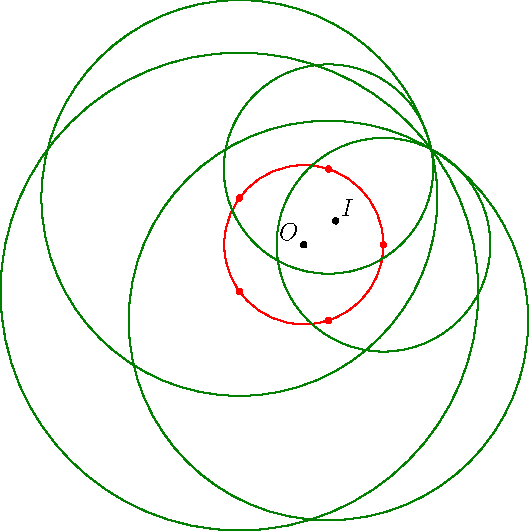
\includegraphics[width=7cm]{./Eintcerc_1.pdf}
 \caption{Cercles $\mathcal{C}_\Omega$.}
 \label{fig:Eintcerc_1}
\end{figure}
On étudie les conditions conduisant à la configuration de la figure \ref{fig:Eintcerc_1} dans laquelle tous les cercles $\mathcal{C}_k$ passent par un même point $M$.
\subsection*{Partie I. Homographie.}
Soit $a$, $b$, $c\neq 0$, $d$ des réels et $h$ l'application de $\R \setminus\{-\frac{d}{c}\}$ dans $\R$ définie par
\begin{displaymath}
 \forall x \in \R \setminus\{-\frac{d}{c}\}:\hspace{0.5cm}
h(x)=\frac{ax+b}{cx+d}
\end{displaymath}
\begin{enumerate}
\item Déterminer en fonction de $a$, $b$, $c$, $d$, des réels $\lambda$ et $\mu$ tels que :
\begin{displaymath}
 \forall x \in \R \setminus\{-\frac{d}{c}\}:\hspace{0.5cm}
h(x)= \lambda + \frac{\mu}{cx+d}
\end{displaymath}
 \item Montrer que $h$ non injective entraine $ad-bc=0$.
 \item Montrer que $ad-bc=0$ entraine $h$ constante et préciser l'unique valeur de $h$ dans ce cas.
\end{enumerate}

\subsection*{Partie II. Analyse.}
 Dans cette partie, on se place dans la configuration de la figure \ref{fig:Eintcerc_1} où tous les cercles se coupent au point $M$.\\
On choisit un repère orthonormé direct $(O,(\overrightarrow i, \overrightarrow j))$ avec $\overrightarrow i =\frac{1}{\Vert \overrightarrow{OI}\Vert}\overrightarrow{OI}$. Les coordonnées de $I$ sont alors notées $(i,0)$ avec $i>0$. Pour tout $\theta$ réel, $\Omega_\theta$ est le point de coordonnées $(R\cos \theta, R\sin \theta)$ dans ce repère.
\begin{enumerate}
 \item Montrer que $M$ est sur la droite $(OI)$. On notera $(m,0)$ les coordonnées de $M$ dans le repère choisi.
 \item Calculer $\Vert\overrightarrow{\Omega_\theta I}\Vert^2$ et $\Vert\overrightarrow{\Omega_\theta M}\Vert^2$.
 \item Montrer que
\begin{displaymath}
 i(R^2+m^2) = m(R^2+i^2) \text{ et } k^2 = \frac{m}{i}
\end{displaymath}
\item Résoudre l'équation d'inconnue $z$ :
\begin{displaymath}
 i^2z^2 - (R^2+i^2)z + R^2=0
\end{displaymath}
\item Quelles sont les valeurs possibles pour $k$ ?
\end{enumerate}

\subsection*{Partie III. Synthèse.}
\begin{enumerate}
 \item Que se passe-t-il si $k=1$ ?
 \item Montrer que si $k=\frac{R}{i}$, tous les cercles $\mathcal{C}_k$ passent par le point $M$ tel que
\begin{displaymath}
 \overrightarrow{OM} = \frac{R^2}{i^2}\overrightarrow{OI}
\end{displaymath}
\end{enumerate}